\documentclass{style/myclass}

\title{System to Classify, Detect and Prevent Hallucinatory Error in Clinical Summarization: An Analysis of 5.4 Million AI-Generated Inpatient Clinical Summaries}
\author{Daniel Kreitzberg, PhD*,Yukun Chen, PhD, Asohan Amarasingham, PhD, Ruben Amarasingham, MD}
\corr{\email{daniel.kreitzberg@piecestech.com}}

\begin{document}

\twocolumn[
\begin{@twocolumnfalse}
\maketitle

\begin{abstract}
Hallucinations—instances where AI models generate inaccurate or unrelated content—pose substantial risks to the summarization of clinical documentation. Yet few frameworks or software methods to reduce these errors have been studied in clinical settings. This technical report introduces the Pieces Classication Framework for Hallucinatory Errors, which utilizes a human-in-the-loop (HITL) platform to categorize and mitigate hallucinations. We analyzed 5.4 million AI-generated inpatient summaries from January 2023 through August 2024 across more than 70 inpatient adult and pediatric clinical specialties. Three nested analyses were conducted to estimate the prevalence of “severe” hallucinations (hallucinations that could lead clinicians to believe emergency interventions are needed for their patients when these interventions are otherwise unnecessary): a global analysis of 5.4 million summaries, a sub-group analysis of 550,297 veriably-reviewed summaries, and a further sub-group of 27,981 manually annotated summaries. Across all analyses, the rate of severe hallucinations was found to be exceedingly low, with 95\% upper condence bounds ranging from 0.402 to 10.7 per 100,000 summaries. We also evaluated the performance of an Adversarial Detection Module (ADM) designed to identify hallucinations of varying severity. 11,108 summaries were manually analyzed, consisting of 827 identied by adversarial detection and 10,281 chosen randomly. The ADM – a necessary component to scale HITL systems – detected clinically signicant hallucinations at a rate 7.5 times higher than cases selected at random. The Eective Remedy Time, the median elapsed time for the HITL system to resolve an AI-generated summary once agged by the ADM for a potential hallucination, was 3.7 hours. These ndings suggest that properly congured clinical AI systems with HITL are capable of classifying, detecting and substantially constraining serious hallucinatory error, demonstrating a promising approach for deploying AI-generated summaries safely and at scale.
\end{abstract}
\vspace{12pt}
\end{@twocolumnfalse}
]	
\section{Introduction to the Pieces Working Summary and the Origin of the Pieces Classication Framework for Hallucinatory Error}

It is widely recognized that the modern-day patient chart has become too long and cumbersome for the time-constrained physician. A typical chart can be half as long as Hamlet, and perhaps more complex.\cite{1} Summarization of the medical record has therefore emerged as a promising and practical use case for AI in medicine. To address this specic need, Pieces Technologies, Inc. introduced the Pieces Working Summary (“Working Summary” or “Summary”), which provides a brief narrative summary of a patient’s hospital course. The Working Summary distills the patient's current status into less than one hundred words – covering the reason for admission, treatments, reasons for continued hospitalization, and upcoming events. The Pieces system monitors the electronic health record (EHR) continuously for updates, and re-writes the Summary when it detects new material information.

One of the critical challenges that arise from generating any type of clinical summary is ensuring its accuracy and reliability. Summaries generated in part by large language models (LLMs) pose certain risks. LLMs are state-of-the-art AI models especially useful for processing textual information. These models are trained on vast amounts of textual data, from which they learn hierarchies of statistical associations among words. These learned associations allow the models to process and produce natural language, including impressive text-summarization capabilities that reect subtle, abstract, and high-order dimensions of the text, such as importance and meaning.\cite{2}

\begin{figure*}
  \centering
  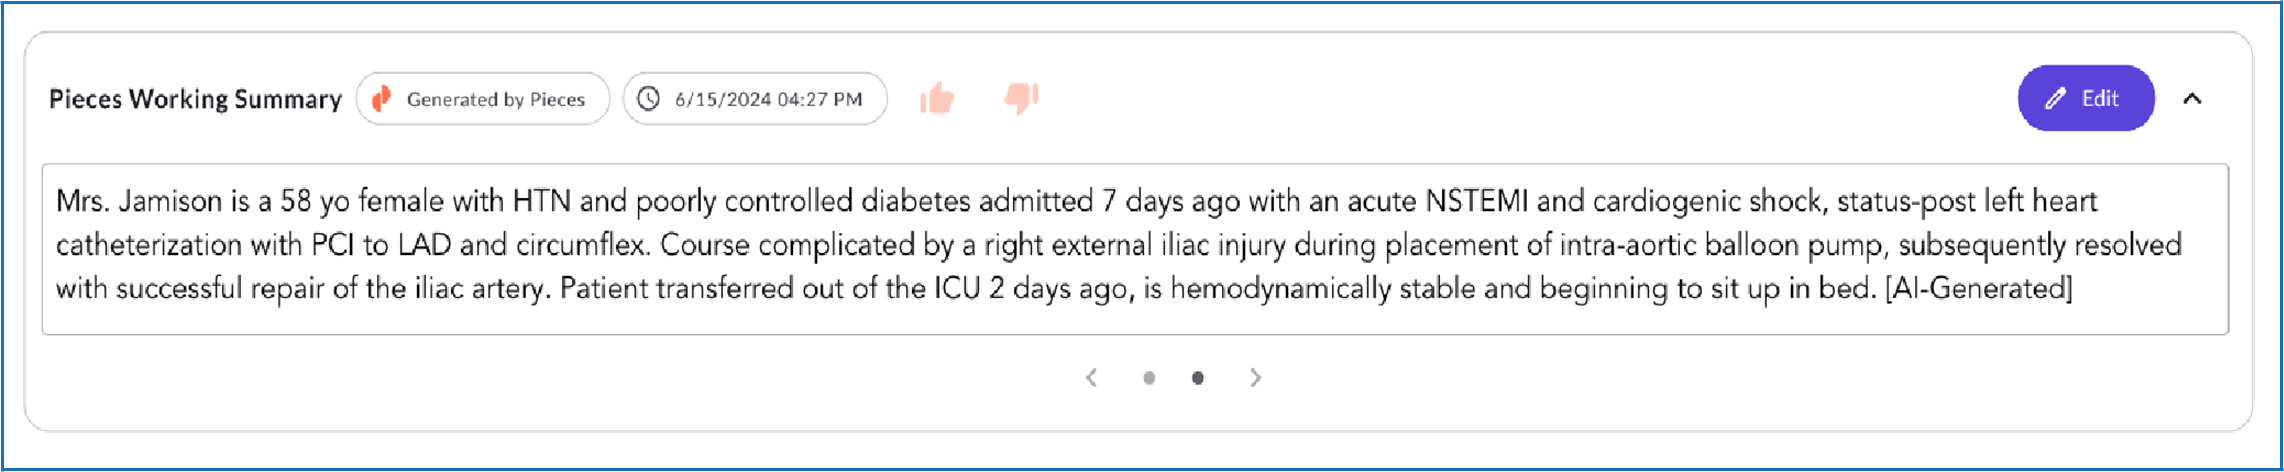
\includegraphics[width=\linewidth]{figure/Picture1.png}
  \caption{\textbf{Example of Pieces Working Summary.} In this 76 word summary, Pieces has drafted a comprehensive narrative summary of what appears to be a complex and somewhat fraught 7-day hospitalization. No matter how complex the case, the Summary is typically brief, designed to be less than 100 words. Therefore, Pieces has to make important judgments regarding what to include and exclude, and the correct level of granularity. The Summary, in its totality, attempts to create a coherent clinical narrative from which the reader can quickly understand the patient context. The information in this example is from synthetic (non-real) data.}
  \label{fig:1}
\end{figure*}

Despite these remarkable capabilities, LLMs have limitations. A signicant limitation is the occurrence of hallucinations—instances where the AI generates new, inaccurate, or unrelated information to the task or source material at hand. The reasons why LLMs generate hallucinations are multifaceted and are themselves a topic of considerable interest among AI researchers. At its simplest level, such errors occur because these systems work by predicting the most likely text that will follow a given input text, according to probabilistic models of language that are learned from massive and general-purpose observational text data. These models may inherit from these training procedures a somewhat limited causal model of underlying knowledge domains. This is a general limitation of LLMs, certainly in current generations, and cuts across elds of expertise.

In specialized areas, such as the clinical data and documentation found in EHRs, the complexity of the subject matter, the potential for missing observations, communication or contexts, and the dangers of inherent errors and corrupted data may increase the propensity for hallucinations within an AI-generated summary, such as the Working Summary. In response to these challenges, Pieces has established a novel set of software and services called “SafeRead” wherein board-certied physicians utilize a classication system specically designed to prevent and categorize the severity of hallucinations within the summary. No suitable frameworks for evaluating inpatient clinical summaries existed, to our knowledge, when we began this work in 2018. We are particularly interested in preventing the most severe of these hallucinations, as we dene it, from reaching clinical end-users as they go about their daily work.

In this paper, we describe the Working Summary; the purpose and methodology behind our new framework, which we describe as the Pieces Classication Framework for Hallucinatory Error (or the “Pieces Framework”); our human-in-the-loop SafeRead platform to evaluate and ensure the Summary is safe to read; the various type of hallucinatory and non-hallucinatory errors and our rationale for focusing on “severe” hallucinations as the rst and most critical objective; and how we estimate the severe hallucination rate using three dierent methodologies. Additionally, we explore the limitations of our classication system, its applicability to other AI-generated clinical documentation such as progress notes and discharge summaries, and outline future directions for research and evaluation, including the role of omissions and lower-severity hallucinations as areas for further investigation.

\section{Definition, Role and Purpose of the Pieces Working Summary and Associated Categories of Error Beyond Hallucination}

 The Working Summary is a concise, 3-4 sentence narrative snapshot of the patient's current status in the hospital. The Summary is modeled after the “Assessment” section of a SOAP note, \cite{3} which is a brief but total summary of the patient’s case including who they are, their relevant past medical history, the working diagnosis or diagnostic di erential, and an update on the evolution of their clinical condition since the beginning of the hospital encounter. This section , sometimes also called the “Impression,” is arguably among the most complex summarization tasks in clinical communication. The Assessment is a remarkable piece of writing when done well. The practitioner must synthesize a potentially vast amount of information from extraordinarily complex cases into a well written summary that does not exceed a few sentences, while faithfully conveying the essence of the case. The Working Summary is intended to replicate the form and substance of the Assessment, while also including key details from the “Plan” section of a typical SOAP note, such as upcoming clinical activities, critical therapeutic milestones, or symptoms and signs to monitor. Unlike a SOAP note, however, which is typically written once per day, the Summary is updated and re-written continuously as new information on the patient emerges 24-hours a day. The intent of the Summary is to allow doctors, nurses, case managers, and administrators to quickly understand and orient themselves to the patient's current situation. An example of a Working Summary is shown in \textbf{Figure \ref{fig:1}.}

The term “Working” is intended to convey that the Working Summary is a “draft” in a number of important ways. The Working Summary borrows from the well known clinical concept of a “working diagnosis,” in which a team may reconsider a current diagnostic hypothesis in the light of new evidence. Similarly, the Working Summary is a point-in-time clinical narrative that evolves as the patient’s course changes and new findings emerge. The Working Summary is considered a draft in the sense that it is not official until accepted or edited by a clinician, nor is it a default part of the legal medical record unless and until a clinician includes it within an officially signed note, such as the History \& Physical, Progress Note, or Discharge Summary.\footnote{We note that the Working Summary does not qualify as a Clinical Decision Support (CDS) medical device under Section IV of the guidance provided in \textit{Interpretation of Criteria in Section 520(o)(1)(E) of the FD\&C Act}. The Working Summary does not provide any analysis or interpretation of medical images, streaming data, or repeated measurements. Instead, it compiles a textual synthesis from existing patient documentation, presenting what is already known without making inferential predictions or interpretations used in diagnosis or treatment. The Working Summary does not direct specific clinical actions such as diagnostics, preventatives, or treatments, but instead relays prior clinical communications and plans it has read in the patient record. The Working Summary remains an editable draft that clinicians can modify and each Working Summary is clearly marked as "AI-generated," underscoring the clinician's autonomy to independently review, edit, or disregard the content as needed. The clinician has the opportunity to refer to all data in the EHR at all times. The Working Summary meets all four of the FDA's exclusionary criteria and as such does not require certification as medical device. I n terms of intended use, the Working Summary is not constructed to provide recommendations or otherwise serve as CDS.}

Displayed prominently within the EHR and clearly marked as AI-generated, the Summary has a number of key uses. \textit{Clinical Handoffs}: First, as previously described, the Summary aims to provide clinicians with a rapid understanding of what has transpired with their patients, reducing time in chart review. Physicians can also edit and use it directly as part of their handoffs to oncoming physicians. Thus, it is especially useful for those covering multiple patient floors or services on cross-cover or weekend shifts. \textit{Reduction in Chart Review Time}: These benefits may especially accrue to case managers, utilization management nurses, administrators, and other non-direct care providers who have a high volume of patients. Working Summaries can reduce time in chart review, prioritize work, and improve team communication. \textit{Supplementation to Clinical Documentation}: The Summary can be inserted into the daily progress note as part of the Assessment section. \textit{Multidisciplinary Rounds}: In these rounds, the Working Summary can support all team members by keeping them informed of the latest patient status, enabling asynchronous communication around patient status, and reducing time in rounds.

\paragraph{Associated Categories of Error}

From January 2023 through August 2024, Pieces Technologies deployed over 5.4 million Summaries across more than 70 inpatient adult and pediatric clinical specialties in a variety of health systems. A key challenge in creating the Pieces Working Summary is determining what information to include or exclude from potentially hundreds to thousands of pages of data, all while preserving the fidelity, temporality, and nuance of each case. In this paper we are primarily concerned with AI-generated Working Summaries that include one type of error, called Hallucination, since it is a type of error particularly unique to LLMs. This emerging type of error is not commonly seen in human clinical summarization unless there is some form of cognitive impairment. Hallucination is an area of key concern for health systems implementing AI systems. \cite{4} We specifically focus on severe hallucinations because the time constraint, criticality to act, and magnitude or potential irreversibility of intervention logically following from this type of hallucination make it the most important type of error, in our view, to prevent.

However, we recognize the importance of other forms of error in comprehension and fluency that humans do very much make, and on which AI systems should also be judged. These include errors of omission (not including the correct facts); errors of misemphasis or mis-prioritization (choosing to highlight less relevant facts over more relevant facts); errors of chronology or completion (incorrect sequence of events, incomplete sentences or unclear ideas), and errors of grammar, syntax, and tense. Moreover, the quality of a summary is not solely defined by the absence of error; excellent summaries must also include positive attributes such as depth, clarity, nuance, and logical coherence. Pieces’ approach to summarization and error handling accounts for these elements, but we will be publishing our findings on these separately from this report.

\section{Establishing a Framework for Hallucinatory Error in the Context of AI-Generated Inpatient Clinical Summaries}

\subsection{Purpose and Objectives of the Classification Framework}

While there is extensive research on AI-generated hallucinations in general situations, \cite{5,6,7} there is limited work classifying the type and severity of hallucinations in the more narrow case of clinical summarization at the point of care. Though the Working Summaries are presented as “AI-generated” drafts to clinicians for their verification, our goal is to reduce or eliminate any serious hallucinatory error before it ever arrives to the clinician. A carefully drawn framework for identifying and classifying such hallucinatory errors serves a number of useful purposes toward this e ort: a) providing a mechanism to grade the severity of the hallucination in order to focus algorithmic and computing e ort on the prevention of the most severe errors; b) o ering a systematic way to identify hallucinations to increase clinician trust in AI systems and to provide a shared language for their documentation; c) using identified hallucinations as feedback to fine-tune the system and reduce future errors; and d) enabling quantification, monitoring and tracking of hallucinations over time.

\begin{table*}
\centering
\begin{adjustbox}{max width=\textwidth}
\begin{tabular}{|C{2.5cm}|L{0.85\textwidth}|}
\hline 
\rowcolor{secblue}
{\color{bg}\textbf{Hallucination Classification}} & \multicolumn{1}{c|}{\color{bg}\textbf{Definition} } \\
\hline 
Severe & 
Non-factual information presented that, if treated as fact, would require emergent (less than 60 minutes) and potentially irreversible interventions that would not otherwise be justified
\\ \hline 
\rowcolor{sbblue}
Major &  Non-factual information presented that, if treated as fact, would require urgent (within the next 24 hours) but not emergent actions that would not otherwise be justified.
\\ \hline 
Moderate & Non-factual information presented or details wrongly emphasized that, if treated as fact, would require actions in 1-2 days.
\\ \hline 
\rowcolor{sbblue}
Minor & Non-factual information presented or details wrongly emphasized. However no treatment was required. \\ \hline 
Any & Any of the above hallucination types. \\
\hline
\end{tabular}
\end{adjustbox}
\caption{\textbf{Definition of Hallucination Types.} Severity classification categories for hallucinations ranging from minor to major were integrated into the SafeRead review process in November 2023. Prior to that, reviewers focused solely on the identification of severe errors. This explains the difference in number of SafeRead reviews analyzed in section 5 below and the number analyzed here.}
\label{tab:1}
\end{table*}

\subsection{Parameters of the Classification Framework}

A successful framework for classifying hallucinations in AI-generated clinical summaries must offer clear, unambiguous definitions that transform the relatively broad concept of hallucination into specific categories that clinical experts can consistently apply. A test of this framework should demonstrate that different reviewers trained on reasonably su cient annotation guidelines, can evaluate the same Working Summary and reliably and e ciently arrive at the same conclusion. To do this we have identified two concepts – which are stark and verifiable and thereby facilitate reviewer training – as the basis for identifying and classifying the severity of a hallucination (see Table \ref{tab:1}). We first establish that hallucinations represent non-factual information that has no evidence or basis in the patient’s medical record. Second, we conclude that the more immediate and critical the clinical response that would logically follow from the hallucinated information, the higher the severity. In this way, hallucinations that would suggest emergency actions—especially those that are di cult to reverse—are classified as the most severe.

Time parameters align with the way clinicians are trained to prioritize tasks based on clinical information, and are more objective – crucial for a reliable classification system. We observed that applying temporality to the classification system significantly improved the consistency of inter-rater classifications. Clinical reviewers were able to make quicker and more confident judgments when given specific timeframes, such as “within 60 minutes” or “within 48 hours,” through which they could assess the urgency of potential actions. In our testing and development, this approach led to higher inter-rater reliability, even with fewer annotation guidelines, because it provides reviewers an intuitive structure that reflects their training in prioritizing tasks based on urgency. For instance, immediate actions such as those involving airway, breathing, and circulation (the “ABCs”) are commonly recognized as something to address in minutes and can be distinguished relatively easily from interventions needed within 24 hours, and this again from interventions within 48 hours. This stratification is outlined in Table \ref{tab:1}.

Severe cases, where the need for immediate intervention might preclude verification, pose the highest risk of harm, while major, moderate and minor cases, as we define them, allow more time for verification and present lower risks of harm to patients. As a general premise, however, we would argue that it would be an exceedingly rare scenario that a clinician would take significant, extraordinary and irreversible action on the basis of a single Working Summary – without confirmatory measures. The goal here then is to “error-proof” the Summary for situations where its purpose is misunderstood or used inappropriately.

\subsection{Evaluating the Framework}

All data used for the analyses described below were collected as part of the normal operations and services of Pieces software; the data was de-identified and aggregated for analyses.

\begin{table*}
\centering
\begin{adjustbox}{max width=\textwidth}
\begin{tabular}{|C{3cm}|C{3.5cm}|C{3cm}|C{3cm}|C{4cm}|}
\hline 
\rowcolor{secblue}
{\color{bg}\textbf{Hallucination Classification}} &  {\color{bg}\textbf{Adversarial Detection $(\mathrm{N}=827)$}} & {\color{bg}\textbf{Randomized Review $(\mathrm{N}=10,281)$}}  & {\color{bg}\textbf{$\mathcal{X}^2(\mathrm{P}$ Value)*}} & {\color{bg}\textbf{IRR\% (95\% CI) [N=50]}} \\ \hline 
Severe & $0(0.0 \%)$ & $0(0.0 \%)$ & NA & $100(93-100)$ \\ \hline 
\rowcolor{sbblue}
Major & $56(6.8 \%)$ & $89(0.9 \%)$ & $202.7(<0.001)$ & $100(93-100)$ \\ \hline 
Moderate & $71(8.6 \%)$ & $169(1.6 \%)$ & $171.2(<0.001)$ & $98.0(89.5-99.6)$ \\ \hline 
\rowcolor{sbblue}
Minor & $43(5.2 \%)$ & $193(1.9 \%)$ & $39.0(<0.001)$ & $98.0(89.5-99.6)$ \\ \hline 
All Hallucinations & $170(20.6 \%)$ & $451(4.4 \%)$ & $376.1(<0.001)$ & $96.0(86.5-98.9)$ \\ \hline 
\rowcolor{sbblue}
No Hallucinations & $657(79.4 \%)$ & $9,830(95.6 \%)$ & $376.1(<0.001)$ & $N$ \\ \hline
\end{tabular}
\end{adjustbox}
\caption{\textbf{Adversarial Detection Module Performance Analysis:} Comparison of Adversarial Detection Module to Randomized Manual Review and Inter-rater reliability scores. A total of 11,108 SafeRead reviews were used to compare the performance of the Pieces Adversarial Detection module for detecting hallucinations with the random sampling approach including 827 adversarial detection AI-flagged reviews and 10,281 randomly sampled reviews. Summaries selected for random review were selected for review through (non-uniform) random sampling (see text). The severity classification categories minor through major hallucinations were integrated into the SafeRead review process in November 2023, hence no data was analyzed here between the period January 2023 through October 2023.*=A Monte Carlo two-sample permutation test, using the chi-squared statistic as the test statistic, was performed on each hallucination category, to test the null hypothesis that adversarial detection and random sampling produced identical distributions of hallucination type. The reported $\mathcal{X}^2$ values provide additional context on the strength of association. Note that the test results are identical for the 'All Hallucinations' and 'No Hallucinations' groups since they are complementary outcomes of the same variable. 95\% confidence intervals around the interrater reliability scores were calculated using the Wilson method. \cite{10}}
\label{tab:2}
\end{table*}


\subsubsection{ Observed Rates of Hallucinations Annotated by Safe Read Physicians}

From November 2023 through August 2024, SafeRead physicians conducted 13,282 reviews of randomly sampled Working Summaries utilizing the Pieces Classification Framework for Hallucinatory Error (with categories ranging from minor to severe hallucinations).\footnote{ SafeRead reviews conducted between January 2023 through October 2023 did not include the full classification framework but only focused on severe errors. The full framework was rolled out in November of 2023, hence N=13,282 for the observed rate in table \ref{tab:2}} SafeRead physicians observed a total of 451 (3.4\%) hallucinations, within this group the majority of these were of moderate or minor severity (n=362, 80.3\%, see Table \ref{tab:2}). In total, 3.4\% of the Summaries contained hallucinations, ranging from 0.7\% for major hallucinations to 1.5\% of reviews for minor hallucinations.

\subsubsection{Inter-Rater Reliability (IRR) of the Classification System}

To assess Inter-Rater Reliability (IRR), or the consistency of hallucination classification across reviewers, we selected a (simple) random sample of two physicians’ reviews of the same 50 summaries (Table \ref{tab:2}). Across these 50 reviews, reviewer A identified two hallucinations (both of moderate severity) while reviewer B also identified two (one moderate and one minor). One moderate hallucination was identified by both reviewers within the same summary while there were two discrepancies between the reviewers: Reviewer A found a minor hallucination that Reviewer B did not annotate and Reviewer B found a moderate hallucination that was not annotated by Reviewer A. This discrepancy resulted in the decrease in IRR for “any” hallucinations.. Thus, the IRR was 96.0\% for any hallucination (regardless of severity), 100\% for severe hallucinations, 100\% for major hallucinations, and 98.0\% for moderate and minor hallucinations. We consider these results preliminary, since it relies on a relatively small sample size of 50 reviews that was not collected specifically for this purpose. Furthermore the underlying prevalence of hallucinations is low, complicating the interpretation of the IRR. Nevertheless, the high agreement percentages are encouraging (see Table \ref{tab:2}) and suggest strong concordance among reviewers.

\subsubsection{Subjective Impressions of the Clinical Reviewers.}

We end this section with a note on the clinical reviewers’ subjective experience with the classification system. The general impressions are that the identification of hallucinations is clear as defined here, that the severity levels are mutually exclusive, and that the time-based criteria assist the reviewer in almost all circumstances to arrive at a final classification.

\section{ Pieces SafeRead: Adversarial Detection Paired with HITL Oversight to Minimize Hallucinatory Error}

Pieces has been actively developing methods to constrain hallucinatory error in clinical summarization for several years. Our approach has culminated in what we call “SafeRead,” which pairs 3 methods: adversarial detection, human-in-the-loop (HITL) control systems, and a curated clinical knowledge graph (see Figure \ref{fig:2}). These methods have been described extensively in the computer science and biomedical informatics literature, and we will not visit their conceptual underpinnings here. In this section we discuss these modules and their relationship to the Pieces Framework

\subsection{Pieces Adversarial Detection Module}

Adversarial detection typically involves identifying and mitigating the efects of inputs that could deceive or mislead AI systems. \cite{8} While traditional adversarial detection focuses on external attacks (e.g. prompt injections), we adapt the terminology to generated outputs. Specifically, our adversarial detection is an AI module (combining both generative AI and other algorithmic approaches) that reviews each generated summary for evidence of inconsistent clinical reasoning predictive of hallucinations, as instructed by a proprietary clinical knowledge graph of summarization errors assembled by Pieces (see Figure \ref{fig:2}). Our approach aligns with recent research that emphasizes the importance of post-generation verification to ensure factual consistency. For instance, Zhou et al. (2021) and Maynez et al. (2020) propose methods for detecting hallucinated content in conditional neural sequence generation by comparing generated outputs with source inputs to identify inconsistencies. \cite{5,6} 

To measure the performance of the Pieces Adversarial Detection Module we examined 11,108 SafeRead reviews, including 827 reviews triggered by the Adversarial Detection Module and 10,281 reviews triggered by random sampling (see Table \ref{tab:2}). A non-parametric permutation test was used to assess whether there is a statistically significant di erence in the proportion of hallucinations identified by the Adversarial Detection Module compared to the random sample review. \cite{9} Specifically, the quantile rank of an observed chi-squared test statistic with respect to the empirical distribution of chi-square statistics generated through Monte Carlo permutations under the null hypothesis gives a p-value for the null hypothesis of no di erence in distribution. Test statistics are reported to provide context on the magnitude of the association.

Adversarial Detection Module reviews had a statistically significantly higher proportion of hallucinations annotated by SafeRead reviewers compared to the random sampling reviews. Specifically, 20.6\% of Adversarial Detection Module reviews found at least one hallucination compared to 4.4\% of random sampling reviews ($\mathcal{X}^2 = 376.1$, $p <0.001$), representing a detection rate 4.68 times higher than that of random reviews. Notably, the detection rate for the most clinically meaningful hallucinations observed (major hallucinations) was 7.5 times higher than that of random reviews. The Adversarial Detection Module reviews had statistically significantly higher proportions of major, moderate, and minor hallucinations random reviews.

The Adversarial Detection Module reviews had statistically significantly higher proportions of major, moderate, and minor hallucinations compared to the random sampling reviews ($\mathcal{X}^2$ ranging from 39.0 to 202.7, all $p <0.001$). While severe hallucinations were not observed, we hypothesized that the Adversarial Detection Module would detect major and moderate hallucinations at a higher rate than in random sampled reviews. The specificity of the Adversarial Detection Module for detecting major hallucinations was 93.0\% [95\% CI=92.5, 93.5] and the sensitivity was 38.6\% [95\% CI=31.1, 46.7] (95\% CI were calculated using the Wilson Method \cite{10}). These results indicate the Pieces Adversarial Detection Module outperforms random sampling for detecting non-severe hallucinations; however, further work is needed to configure and improve sensitivity specifically for non-severe error types.

\subsection{Pieces Clinical knowledge graph (“knowledge graph”)}

Pieces has developed a proprietary knowledge graph that informs Summary generation in a process called “grounding”. Grounding means ensuring the model is accessing specific, trusted and verified data sources when generating output, as opposed to purely relying on pre-trained language models without internal knowledge. \cite{11} Pieces’ selection of data for input into the Summary generation module is similar in part to a retrieval augmented generation (RAG) system method by retrieving task relevant document windows from EHR records as the input to LLMs. \cite{12,13} However, Pieces chooses its extraction of the record based on the instruction of the knowledge graph. As a result, the system processes a smaller, more relevant portion of the health record data at any given time. Narrowing the input window has been shown to reduce noise and complexity in input systems that might otherwise lead to hallucinations, as long as window selection is accurate. \cite{14} This approach has the added benefit of cost and computational efficiency.

The knowledge graph also serves as a framework for the adversarial system to verify AI-generated content against both a) verified sources in the patient’s record and b) curated clinical content that Pieces assembles from peer reviewed clinical literature, HITL annotations, end-user edits, and direct client feedback (see Figure \ref{fig:2}). Since new clinical concepts found in the annotations are input into the knowledge graph, the system’s capacity for detecting hallucination, or other errors, grows over time promoting scalability. Researchers have used similar approaches for constraining both intrinsic hallucinations (in which the generated text is contradicted by internal knowledge, e.g., knowledge internal to the EHR) and extrinsic hallucination (in which internal knowledge is not sufficient to recognize the hallucinatory error) among chatbot conversation responses.\cite{11}

\subsection{Pieces Human-in-the-Loop (HITL) Control System: “SafeRead”}

HITL control systems refer to AI systems that incorporate human oversight at key stages of an AI’s decision-making process. HITL systems have been used to safeguard against potential model errors in high-stakes situations, such as semi-autonomous driving, by allowing humans to intervene and correct AI-generated decisions. The interventions themselves then become a training set for further improving the model, possibly towards the ambition of full autonomy.

Pieces HITL, called “SafeRead”, is built on a similar principle (see Figure \ref{fig:2}). The SafeRead system revolves around board certified physicians – expert clinical reviewers – who are trained in the Pieces Framework and are empowered to intervene as the final quality control in detecting and mitigating hallucinations before the Summary arrives to end-users. The adversarial detection module first flags Summaries that have a high potential for hallucinations and assigns them to an expert reviewer for evaluation. SafeRead reviewers utilize specific annotation guidelines evaluating each clinical summary for accuracy and completeness, making edits when necessary. Clinicians reviewing these flagged cases can either approve, reject, or edit the Summary based on their professional judgment. After editing, they document the reasons for their changes by selecting the applicable annotation categories (e.g., diagnosis, procedure, medication), specifying the severity level and type of error encountered, such as hallucination, omission, or other (e.g. stylistic issue, duplication, etc), according to the Pieces Framework. A view of the SafeRead annotation screen is depicted in Figure \ref{fig:3}. The SafeRead platform is also used to conduct reviews selected at random.

\subsection{Effective Remedy Time}

We define the “Effective Remedy Time” as the median elapsed time for the system to resolve a Summary when it is flagged by the adversarial detection module for a potential severe hallucination. Using data from July 20\textsuperscript{th} through August 25\textsuperscript{th}, 2024, which represented the period corresponding with the latest version update to the Adversarial Detection Module (Summaries n=689,768), the median Effective Remedy Time was 3.7 hours (n=1,738). There are 2 sub-classes of flagged Summaries with respect to Remedy Times. In the first class are the flagged Summaries that are resolved by SafeRead clinician reviewers. The “Human Remedy Time” is the median time to review for the human-reviewed flagged Summaries, which was 12.2 hours (n=452). However, since the system is continuously generating new Summaries based on updated information, the system will allow a new Summary to replace a flagged Summary if permitted by the adversarial detection module. We define the “Machine Remedy Time” as the median time to resolution among these machine-resolved flagged Summaries, which was 2.7 hours (n=1,286).

\subsection{Random Sampling Procedure}

We also reviewed random samples of Summaries across the client base, downstream of the adversarial detection module (see Figure \ref{fig:2}). The Summaries to be reviewed were sampled disproportionately across hospital lines to ensure adequate representation of reviews from diverse hospital service lines, including those with smaller patient populations. This approach was used for quality control to ensure that units with lower patient volumes also received sufficient SafeRead reviews, but the sampling procedure was constrained only by patient volume and was not designed in light of any known dependency between service lines and hallucinations. This (non-uniform) random sampling procedure is a complement to the Pieces Adversarial Detection Module as it can, in principle, catch a broader range of hallucination patterns than the adversarial detection was designed to detect. Further, random sampling can separately evaluate and inform the performance of the Adversarial Detection Module. If hallucinations are consistently identified in the non-uniform random sample but missed by the algorithm, the algorithm could be adjusted. Additionally, adversarial detection may struggle with "edge cases" or rare scenarios that occur infrequently in the data, possibly among smaller patient populations with more complex clinical cases, due to lack of prior examples.

\begin{figure}[t]
    \centering
    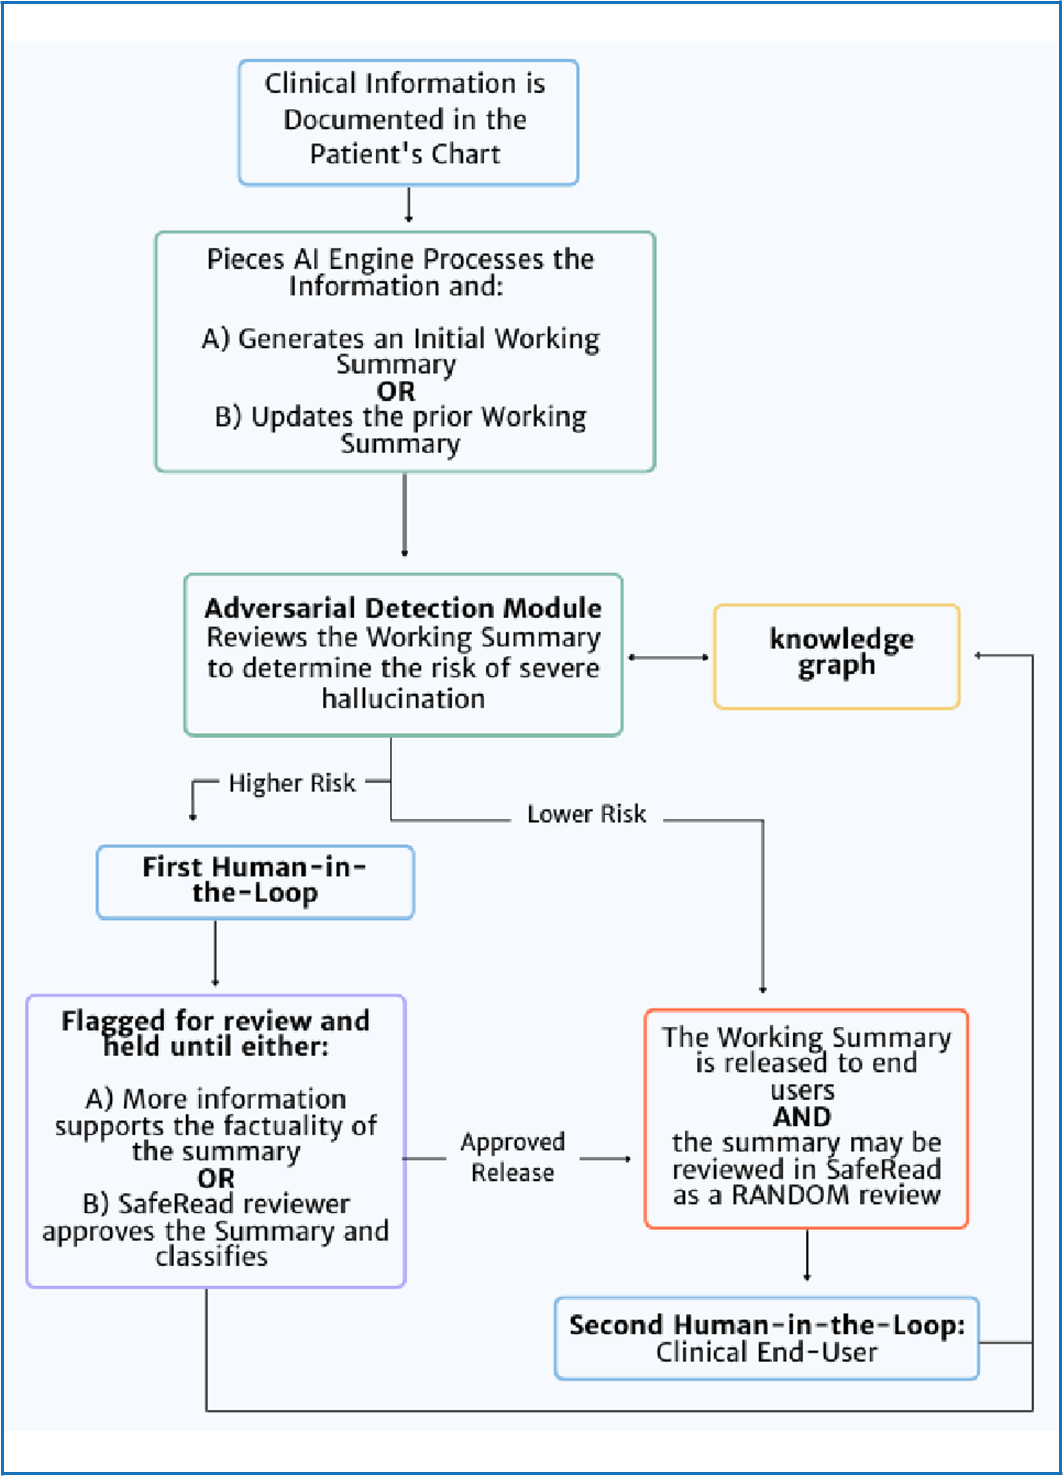
\includegraphics[width=\linewidth]{figure/Picture2.png}
    \caption{\textbf{SafeRead System to Classify, Detect, and Prevent Severe Hallucination.} This diagram illustrates the process for classifying, detecting, and preventing severe hallucinations in the Working Summary. An adversarial detection module (ADM) scans each summary using a clinical knowledge graph to validate content against patient records and curated clinical sources. Two human-in-the-loop stages follow: (1) SafeRead physicians review ADM-flagged high-risk summaries, and (2) clinical end-user feedback and edits. SafeRead physicians also classify other errors, including omissions, misemphasis, chronology, and stylistic issues.}
    \label{fig:2}
\end{figure}

\begin{figure*}[t]
\centering
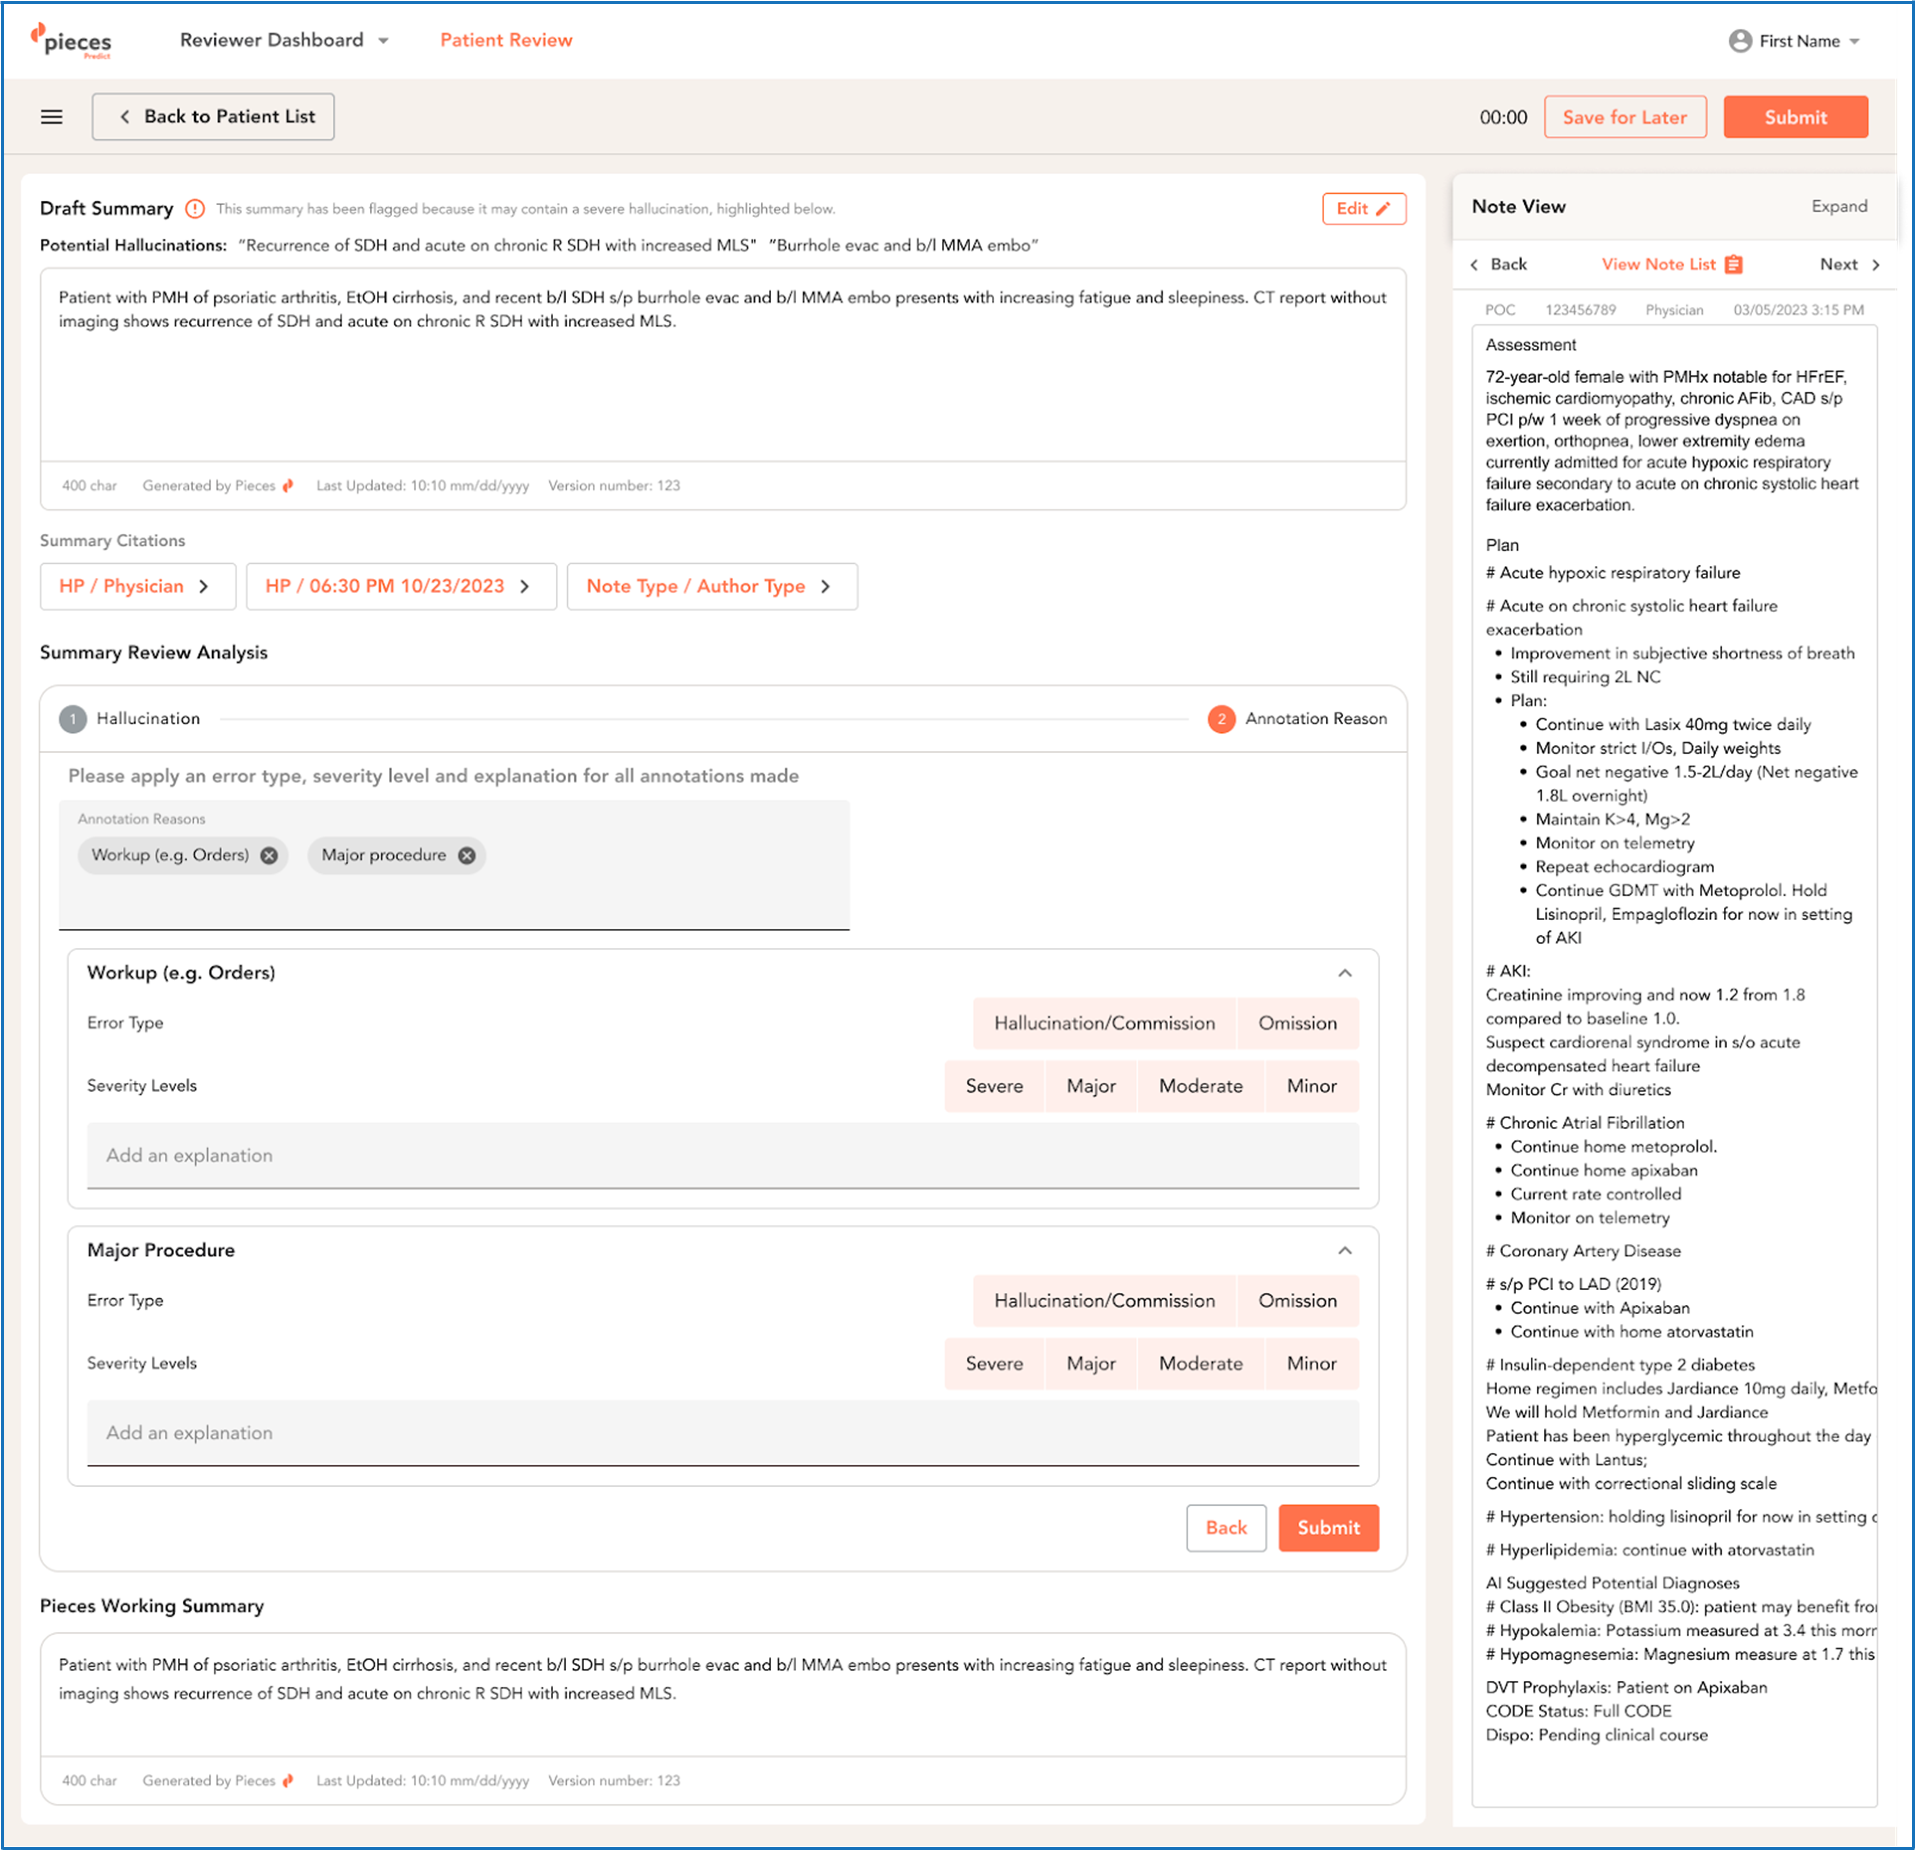
\includegraphics[width=0.7\linewidth]{figure/Picture3.png}
    \caption{\textbf{Screenshot of the Pieces Human-in-the-loop SafeRead Platform.} The content included in this screenshot is synthetic (not real) data. In this secure, encrypted, HIPAA compliant system, clinical data are presented alongside Pieces AI output enabling board-certified expert physician reviewers to validate AI conclusions. In this example, SafeRead reviewers annotate the particular error found (e.g., in a major procedure, as seen above), the type of error (e.g. Hallucination or Omission), and the severity of the given error. Reviewers may identify multiple errors per review. These errors are additionally used to retrain the adversarial detection system in a system of continual improvement.}
    \label{fig:3}
\end{figure*}

\section{Analysis of Severe Hallucinations Rates within the Working Summary}

Estimating the rate of severe hallucination helps forecast the reliability and performance of the Pieces Working Summary at scale. Here we establish and interpret confidence intervals (confidence upper bounds) for the probability of severe hallucination according to our latest data, elucidate their underlying assumptions, and discuss caveats. To approach this problem, we decided to consider the estimated rate using three different baskets of Summaries, each analyzed with a different set of assumptions and limitations: a) a global analysis of the full set of 5.4 million Summaries generated with an unknown level of review; b) a more limited set of 550,297 Summaries that were known to be reviewed; and c) 27,981 Summaries that underwent detailed clinical review with annotation according to the Pieces Framework.

\subsection{Analysis of 5.4 Million Summaries}

From January 2023 through August 2024, Pieces generated approximately 5.4 million Working Summaries across our client health systems. During this period we collected all known hallucinations identified by our clients in one of three categories: 1) hallucinations identified from edits to the Summary by clinical end-users; 2) hallucinations flagged by clinical end-users using our user support ticketing system; and 3) direct feedback from clients in weekly touchpoints and governance sessions. Each case was then subsequently evaluated by physician staff at Pieces for the evidence of a severe hallucination by a clinical review team according to the Pieces Framework. Zero of these cases were ultimately classified as severe. That is, the observed rate of severe hallucinations was 0\%. However, we cannot conclude from this observation that the true rate is 0\%, because we need to account for sampling variability, as well as the process by which severe hallucinations, once generated, would come to our attention.\footnote{See also Section 2 of the Appendix for further discussion of the role of theoretical and observable quantities in statistical modeling.}

The Working Summary is displayed in a user’s patient list directly within the electronic health record. The patient list contains several columns of information, such as the patient name, medical record number, hospital bed, and administrative data. As such, when users login to that view, Pieces does not have insight into whether a specific Summary has actually been read, or how thoroughly it has been read. So, in this circumstance, in order to estimate the true rate, we need to apply some reasonable assumptions concerning the likelihood that a severe hallucination would come to Pieces’ attention.

Let us call $c$ the (conditional) probability that a Summary will come to the attention of Pieces, given the knowledge that it contains a severe hallucination. (In other words, $c$ is the probability that a Summary, drawn randomly from the population of Summaries containing a severe hallucination, will come to Pieces’ attention.) It will be useful for the subsequent analysis to have a lower bound c L for $c$ satisfying $c \geq c_L$ . We reason that a reasonably conservative lower bound for $c$ is 0.1379, based on the following facts and mildly conservative assumptions: a) we assume that no more than approximately 50\% of the Summaries generated are candidates for viewing, and thus reporting. Our internal data and prior research show that the majority of EHR activity is concentrated during day time hours (between 7 am and 7 pm) when 50\% of the Summaries are generated. (The median number of Summaries generated per patient per day is 4). \cite{15,16} b) We assume the number of clinical staff per case (including physicians, nurses, and case managers) is 5 \cite{16,17} , $c$) though extensive efforts are made to educate staff, we assume that no more than 25\% of all the eligible clinical staff are familiar enough and using the Summary, a conservative estimate, which is less than our experiences in the field would suggest, \cite{18,19} d) a lower bound of 25\% of staff would report a given severe hallucination within the Summary, once identified, based on our experience and related literature. \cite{20} Assuming that these factors act (conditionally) independently of one another and of the fact of a severe hallucination, this results in a lower bound of $c_L =0.1379$ for the conditional probability $c$. (The conditional independence and plugin assumptions are a reasonable first-order approximation given the evident sparsity of severe hallucinations.)

\begin{table*}
\centering
\begin{adjustbox}{max width=\textwidth}
\begin{tabular}{|C{2.5cm}|C{4cm}|C{10cm}|}
\hline 
\rowcolor{secblue}
{\color{bg}\textbf{Analysis}} & {\color{bg}\textbf{Summaries Analyzed}} & {\color{bg}\textbf{Severe Hallucination Rate: 95\% CI Upper Bound}} \\
\hline 5.1 & $5,400,000$ & $<1$ per 100,000 \\
\hline 5.2 & 550,297 & $\leq 1.088$ per 100,000 \\
\hline 5.3 & 27,981 & $\leq 10.7$ per 100,000 \\
\hline
\end{tabular}
\end{adjustbox}
\caption{\textbf{Analyses of Severe Hallucination Rates Across 3 Samples of Summaries.} Estimated rates of severe hallucinations using three different baskets of Summaries, each analyzed with a different set of assumptions and limitations: a) a global analysis of the full set of 5.4 million Summaries generated with an unknown level of review; b) a more limited set of 550,297 Summaries that were known to be reviewed; and c) 27,981 Summaries that underwent detailed clinical review with annotation according to the Pieces Framework.}
\label{tab:3}
\end{table*}

What is the theoretical implication of the fact that 0 severe hallucinations have come to our attention out of a large number (n=5.4M) of Summaries? We use that observation to infer the probability $p$ that a \textit{random sample}  would include a Summary with a severe hallucination. (Among other examples, this random sample could model a new summary that arrives from the same process that generated the data.) This is done by regarding the Summaries as independent samples from a common probability distribution. Under these assumptions, we obtain a 95\% confidence interval of [0, 0.00000402) for the probability of severe hallucination assuming the probability of failure to identify or report a severe hallucination is 86.21\% or less (see Technical Appendix).\footnote{See Section 1 of the Technical Appendix for a derivation of the confidence interval formulae used in this section. In this application, the lower bound for $c$ is $c_L =13.79\%$, $\alpha=0.05$, and $\theta$ is the probability of a severe hallucination coming to the attention of Pieces. The CI derives from the fact that $\theta \geq pc_L$ .} That is, we can \textit{rule out} that the probability of severe hallucination is greater than 0.402 per 100,000 summaries, under these assumptions with 95\% confidence (see Table \ref{tab:3}). Equivalently, we expect, by this reasoning and assumptions and with 95\% confidence, an average of no more than .402 severe hallucinations per 100,000 summaries. (The observed data [0 observations] is compatible with a lower rate, but a rate as high as .402 severe hallucinations per 100,000 cannot be ruled out with as much as 95\% confidence.)

\subsection{Sub-Group Analysis of 550,297 verifiably-reviewed summaries}

Users who would like a more detailed review of the Working Summary are able to double-click on the Summary in the patient list view to see more detail and additional patient context features, including viewing prior Summaries in reverse chronological order to obtain a narrative timeline of the patient. In this sense, the act of navigating to this view of the Summary itself verifies that the Summary has been reviewed, which we call a “verifiably-reviewed Summary.” From January 2023, through August 2024, 550,297 Summaries were verifiably-reviewed. With this data we can model $c$, the (conditional) probability that a summary will come to the attention of Pieces, given the knowledge that it contains a severe hallucination, with fewer assumptions.

Here, we reason that a lower bound for c is 50\%, based on a single assumption: a) we assume that 100\% of the clinical staff who are using the Pieces navigator are familiar enough with the technology to edit or report a severe hallucination since they specifically navigated to the Summary within the EHR; and we estimate b) at least 50\% of this staff would report a severe hallucination (a two-fold increase from the scenario in section 5.1) if they found one, using one of the three mechanisms to report such a hallucination. \cite{20} The increased probabilities for assumptions a) and b) derive from our experiences interacting with clinical staff who actively use the Pieces Summary view in the EHR, who we consider “super-users” of the software. \cite{21}

Under these assumptions, we obtain a 95\% confidence interval of [0, 0.00001088) for the probability of severe hallucination within the population of verifiably-reviewed summaries, assuming the probability of failure to identify or report a severe hallucination is 50\% or less (see the Technical Appendix). Equivalently, we expect, by these assumptions and reasoning and with 95\% confidence, an average of no more than 1.088 severe hallucinations per 100,000 verifiably-reviewed Summaries (see Table \ref{tab:3}).

\subsection{Sub-Group Analysis of 27,981 SafeRead reviews}

We also have a subgroup of 27,981 Summaries that were manually reviewed by board-certified physicians in our SafeRead system. We observed 0 severe hallucinations in this subgroup comprising both 16,903 Summaries flagged by random sampling and 7,371 Summaries flagged by the adversarial detection system for review. Again, we infer from this data set the probability $p$ that a random sample would include a Summary with a severe hallucination. (The statistical reasoning is as in Section 5.1 above, but in this application the quantity $c$ is assumed to be 1 by definition.) Applying this model to the SafeRead evaluations, a 95\% confidence interval for this \textit{probability of severe hallucination} would be [0, 0.000107). Equivalently, one would expect, based on this data and with 95\% confidence, an average of no more than 10.7 severe hallucinations per 100,000 summaries (see Table \ref{tab:3}). (\textit{The observed data is compatible with a lower rate, but a rate as high as 10.7 per 100,000 cannot be ruled out with as much as 95\% confidence.})

Because of the sampling procedure, we can re-interpret this as the probability that a random sample selected using the above statistical mixture of the adversarial detection process and the random selection process (see Section 4.5) contains a severe hallucination. The sampling procedure and the adversarial detection system were not designed with any known bias towards selecting cases that would be less likely to generate a hallucination within a Summary. In fact, the adversarial module outperforms random sampling for detecting Summaries with hallucinations of varying severity levels (see Table \ref{tab:2}). Given the use of a mixture of the adversarial detection system and random sampling for flagging Summaries for review, it is thus also plausible that the confidence interval would either approximately obtain for, or more likely even be conservative for, a simple random sampling approach.

\subsection{Summary of Analyses}

By leveraging three different nested data sets, we can estimate upper bounds on the rate of severe hallucinations in the Pieces Working Summary under different modeling assumptions (see Table \ref{tab:3}).

In the Global Analysis (5.4 million Working Summaries), which is based on reports from clinical staff and feedback channels across client systems, we estimate an upper bound of 0.402 severe hallucinations per 100,000 summaries with 95\% confidence. This estimate, $<1$ per 100,000, includes relatively conservative assumptions implicating the likelihood that a hallucination would be reported and visible to Pieces.

The Sub-Group Analysis of Verifiably-Reviewed Summaries (550,297 summaries) has fewer assumptions. In this case the summaries were “verifiably reviewed” through the Pieces navigator: here we obtain an upper bound of 1.088 severe hallucinations per 100,000 verifiably-reviewed summaries with 95\% confidence.

Finally, the Sub-Group Analysis of SafeRead Reviews, which involved manual review by board-certified physicians, observed no severe hallucinations in 27,981 Summaries. This subgroup analysis provides a robust confidence interval that suggests an upper bound of 10.7 severe hallucinations per 100,000 summaries with 95\% confidence, a more cautious estimate because no assumptions are made about the process through which severe hallucinations are reported, the manual review is more costly, and we do not account for the conservative effect of the adversarial detection process.

These approaches provide complementary views of the system’s performance under different sample sizes and attendant assumptions. Taken collectively, the analysis provides strong evidence that the rate of severe hallucination is very low.

\section{Discussion}

We have chosen a narrow area of focus for error classification within the specialized domain of AI-generated inpatient clinical summaries — namely, the concept of hallucinations. We do so because hallucinations are a prominent type of error introduced by the emergence of large language models (LLMs); this type of error is not commonly seen in human clinical summarization unless there is some form of cognitive impairment. Hallucinations represent an important area of concern for health system leaders implementing AI systems. \cite{4} In this paper, we specifically focus on severe hallucinations, as we define them, because the time constraint, criticality to act, and magnitude or potential irreversibility of intervention logically following this type of hallucination make it the most important type of error to prevent.

We present here both a framework and method to classify, detect and prevent severe hallucinations. Across a large sample of AI-generated summaries (N=5.4 million) on a large and diverse health system base using the Pieces summarization method, we observed zero severe hallucinations. From this data, we estimate that this method generates a very low true (i.e., under the model, see S.2 of Technical Appendix) rate of severe hallucination according to three distinct analyses (ranging from $<1$ per 100,000 to no more than 11 per 100,000 summaries). Some might argue that the threshold to meet a severe hallucination (a hallucination that could lead clinicians to believe emergency interventions are needed for their patients when these interventions are otherwise unnecessary) is so high as to make the achievement less meaningful. We would disagree with this logic as these clinical events are by nature rare and serious. However, we also found that the next temporal category of “Major” hallucinations, those hallucinations that would support treatment within 24 hours, is also rare: 0.9\% of manually classified summaries. These results suggest that the summarization approach we have outlined, or elaborations in its direction, may have promise to effectively constrain the most critical forms of hallucination.

\subsection{Limitations}

While we feel that this analysis is informative, it is not without limitations. First, we used a number of modeling assumptions to derive the estimated severe hallucination rates in analyses 5.1 and 5.2. The quality of these assumptions may affect the accuracy of our estimates. For example, in both of those analyses we assume a certain willingness to report or edit a severe hallucination rate among the clinicians; if the real willingness is lower than that proposed, we may be underestimating the true rate of severe hallucination. To address this, we conducted three distinct analyses, with each analysis reducing the set of assumptions. Our third method of estimation, though a smaller sample size overall, did not require any additional assumptions. We are encouraged by the fact that all 3 analyses point to a very low severe hallucination rate.

To address this methodologic challenge in the future, we are adding monitoring capabilities to Pieces that would allow us to replace those assumptions with actual observational data on the specific user behavior in question. Such monitoring might also facilitate a better understanding of how user behavior is affected by onboarding, training, and workflow design, ultimately leading to better user designs and in turn more refined estimates of hallucination and other error rates. Second, our preliminary results suggest high inter-rater reliability (IRR) between reviewers using the Pieces Classification Framework. The sample size is small however and in a setting where the overall prevalence of (even moderate and minor) hallucinations appears to be low. Thus the IRR we present may be overstated. Calculation of the IRR here is challenged by the fact that the original data collection was operational in nature and not designed specifically for this analysis. We plan to conduct future IRR analyses with larger sample sizes, across a greater range of clinical specialty types and domains of error, prospectively, and with research grade data. Third, our sampling scheme for selecting summaries to review was not uniform by design, in order to detect hallucination errors across a broader range of clinical service lines. Non-uniformity may contribute some unknown bias to the estimate derived from this random sampling procedure. In the future we will include parallel approaches that include uniform random sampling or explicitly correct for nonuniform sampling. Lastly, the analysis was conducted on summaries generated between January 2023 through August 2024; the summaries during this period were treated uniformly. However, the software underlying the Working Summary incorporated several iterative improvements in both the underlying algorithm and external user interface as it advanced from generation 7 to generation 10. This may have had unknown effects on the error handling that make projections harder to generalize. As a general proposition however, we would expect these advances to improve, rather than worsen, the error rates over time. This highlights the need, recommended elsewhere, to continuously monitor error rates as a part of a standard safety practice for dynamic AI programs. \cite{22}

\subsection{Future Directions}

As we have remarked, hallucinatory error is not the only error type one would need to monitor and prevent in an AI-generated summary. Additional errors arise in comprehension and fluency that humans very much make, and on which AI systems should also be judged. These include errors of omission (not including the correct facts); errors of misemphasis or mis-prioritization (choosing to highlight less relevant facts over more relevant facts); errors of chronology or completion (incorrect history, incomplete sentences or unclear ideas), and errors of grammar, syntax, and tense. Moreover, the quality of a Summary is not solely defined by the absence of error; an excellent clinical summary must also include positive attributes such as depth, clarity, and logical coherence. We have extended the error framework presented here to include these additional domains of error and will publish separate findings on each of these. For example, we have found that parameters in this framework extend well to the concept of omissions. Summaries by nature must omit information in order to achieve the act of summarization itself, but removing the wrong information will drastically affect the essential truth or meaning of the summary. Organizing errors of omission under the same framework of time and magnitude of interventions shows promise according to early data.

We are also working on evaluating our generative AI output through traditional capability based assessments such as the PDQI-9 (Physician Documentation Quality Instrument-9). Though this assessment does not measure hallucinatory errors, it does evaluate other dimensions such as the completeness, accuracy, organization, and overall quality of documentation made by physicians in medical records. Early results comparing the Working Summary on these more affirmative measures of quality are positive. This peer-reviewed methodology may be complementary to the Pieces Framework and might be useful for judging a broad range of AI-generated note types beyond summarization including progress notes, transfer notes, discharge summaries, and lifetime medical summaries. This is being studied now.

\section*{Acknowledgement}

We extend our deepest gratitude to the many stunning teams and individuals at Pieces Technologies who contributed to GEN10 of the Pieces Working Summary. Special thanks to our: AI, Software Engineering, and Product teams for their craftsmanship; our SafeRead and AI Safety teams for standing guard, and for our IT infrastructure, privacy and SecOps teams for keeping us and our clients safe; our operational teams, including our executive assistants, finance, recruitment, and legal for empowering our entire company to perform at its best; our professional services, client success, marketing, and communications teams for reaching our customers and telling our story. We appreciate our health system clients and partners – without you we could not do any of this. Thank you for your essential role in refining our technologies, your candor, your ideas, your fundamental commitment to serving patients and their families.

Please cite this work as “Pieces Technologies Inc., System to Classify, Detect and Prevent Hallucinatory Error in Clinical Summarization: An Analysis of 5.4 Million AI-Generated Inpatient Clinical Summaries (Technical Report 10.2024)”

\section*{ABOUT THE AUTHORS}

\textbf{Daniel Kreitzberg, PhD}, is the Director of AI Safety and Clinical Effectiveness at Pieces. He received his PhD in Health Behavior and Health Education from the University of Texas at Austin. Dr. Kreitzberg’s applied and research interests are focused on evaluating generative AI's impact on health system efficiency and user behavior; leveraging AI to harmonize disparate EHR data sources for longitudinal tracking of patient care; scalable adversarial AI monitoring of patient chatbot conversations; and AI safety. He is an NIH-funded investigator and published on topics of real world data analysis, health communication and user behavior.

\textbf{Yukun Chen, PhD}, is the Vice President of Artificial Intelligence (AI) at Pieces. Dr. Chen received a Masters in Electrical Engineering from the University of Pennsylvania and PhD in Biomedical Informatics from Vanderbilt University. His dissertation focused on the application of active learning to clinical NLP tasks, and human-in-the-loop interactive machine learning systems. Dr. Chen’s research interest is in applied generative AI methods, active learning, and human-machine collaborative learning. He has published over 20 peer-reviewed papers including in \textit{Nature Methods, JAMIA, JBI}, and others journals in biomedical informatics.

\textbf{Asohan Amarasingham, PhD}, is a Principal Mathematician at Pieces and Professor in Departments of Mathematics, Computer Science, and Biology at the City College of New York and the Graduate Center of the City University of New York. He received his PhD in Applied Mathematics from Brown University. His main areas of scientific interest are in statistics, machine learning, and theoretical and experimental neuroscience. Dr. Amarasingham’s scientific work has been supported by lead investigator grants from NSF, NIH, DOE, and ARO, among other agencies, and has appeared in Science, \textit{Proceedings of the National Academy of Sciences, Uncertainty in Artificial Intelligence, Neural Computation, and Nature Neuroscience}, and other primary research journals.

\textbf{Ruben Amarasingham, MD}, is Founder and CEO at Pieces. He has received degrees and post doctoral training from Brown University, the University of Texas Southwestern Medical Center, and the Johns Hopkins Medical Institutions. Dr. Amarasingham’s research has focused on clinical predictive models and the development and evaluation of technology to improve quality of care and reduce disparities. His research has been supported by the NIH, NCI, NSF, the Robert Wood Johnson Foundation, the Gordon and Betty Moore Foundation, the WW Caruth JR Foundation and the Commonwealth Fund. He has published original research in the \textit{New England Journal of Medicine, JAMA Archives, BMJ Quality \& Safety, JAMIA, Medical Care} and other journals in biomedical informatics and health services research.

\printbibliography

\titleformat{\section}{\normalfont\fontsize{11}{14}\selectfont\bfseries\raggedright}{\thesection}{1em}{#1}
\titlespacing\section{0pt}{12pt plus 4pt minus 2pt}{12pt plus 0pt minus 0pt}
\titleformat{\subsection}{\normalfont\bfseries\raggedright}{\thesubsection}{1em}{#1}
\titlespacing\subsection{0pt}{12pt plus 0pt minus 0pt}{12pt plus 0pt minus 0pt}
\titleformat{\subsubsection}{\normalfont\bfseries\raggedright}{\thesubsubsection}{1em}{#1}
\titlespacing\subsubsection{0pt}{12pt plus 0pt minus 0pt}{12pt plus 0pt minus 0pt}
\titleformat{name=\section,numberless}[block]{\normalfont\fontsize{11}{14}\selectfont\bfseries\raggedright}{}{0em}{{#1}}
\setcounter{section}{0}
\setcounter{footnote}{0}
\setcounter{figure}{0}
\setcounter{table}{0}
\setcounter{page}{1}

\onecolumn
\pagestyle{appendix}

\newcommand{\Appendixhead}{
\begin{center}
\LARGE\textbf{Technical Appendix}
\end{center}
}

\Appendixhead

\section{Confidence intervals for a binomial proportion}

We review some basic concepts from theoretical statistics as necessary; see [1] for a thorough treatment. Let $\theta$ be the probability of a binary event (e.g., severe hallucinations that come to our attention), and $X$ the number of times the event occurs in $n$ independent samples. We seek a confidence interval for $\theta$ in this binomial sampling model. It is interesting to note that this problem continues to stimulate discussion and innovation in the statistics literature (see [2] and its ensuing discussion). For example, the Wald interval has been strongly disavowed, but only relatively recently [2]. It appears to us that much of this debate stems from various disagreements about the purpose of the interval, suggesting that its resolution should ultimately be decision-theoretic. This is worth keeping in mind when interpreting the intervals in our discussion. For our purposes in the attached report, the one-sided Clopper-Pearson interval, which arises by inverting tests of the form $\left\{X \leq k_{\theta}\right\}$, where $k_{\theta}$ is determined by the hypothesized $\theta$, is compelling - possibly, uniquely so. [4,5] give arguments and evidence in favor of the last point.

\subsection{Confidence Interval for $\theta$}

For completeness, the (one-sided) Clopper-Pearson interval is constructed as follows. Fix $\alpha \in(0,1)$. A size $\alpha$ test of the hypothesis $H_{0}: \theta=\theta_{0}$ is provided by the critical region $\left\{X \leq k_{\theta_{0}}\right\}$ where
\begin{equation}\label{eq:1}
k_{\theta_{0}}:=\max \left\{k \in\{-1,0, \ldots, n\}: P_{\theta_{0}}(X \leq k) \leq \alpha\right\}, 
\end{equation}

meaning that $P_{\theta_{0}}\left(X \leq k_{\theta_{0}}\right) \leq \alpha.$\footnote{-1 is included in the range that $k$ is maximized over for bookkeeping reasons. $k_{\theta}$ will be -1 when there is no size $\alpha$ critical region in this form except the empty set.} Note that the test is 'one-sided': targeting alternatives where $\theta$ is smaller than the null hypothesis. More colloquially, the tests ask: 'Is $X$ suspiciously small for $H_{0}$ ?'. It is the textbook test for these alternative hypotheses.

The set of all hypotheses that the data $X$ fails to reject at level $\alpha,\left\{\theta^{\prime}: X>k_{\theta^{\prime}}\right\}$, is a level ( $1-\alpha$ ) confidence interval for $\theta$. That is, $P_{\theta}\left(\theta \in\left\{\theta^{\prime}: X>k_{\theta^{\prime}}\right\}\right) \geq 1-\alpha$ under the binomial sampling model. This is because, by construction, $P_{\theta}\left(X \leq k_{\theta}\right) \leq \alpha$ for all $\theta$. Constructing an interval from a family of hypothesis tests in this way is called 'inverting' the tests.

When the data $X$ takes the value 0 , this interval takes a simple closed form:

\begin{align}
\label{eq:2}
\left\{\theta^{\prime}: X>k_{\theta^{\prime}}\right\} & =\left\{\theta^{\prime}: 0>k_{\theta^{\prime}}\right\} \\
\label{eq:3}
& =\left\{\theta^{\prime}: P_{\theta^{\prime}}(X=0)>\alpha\right\}=\left\{\theta^{\prime}:\left(1-\theta^{\prime}\right)^{n}>\alpha\right\}=\left\{\theta^{\prime}: \theta^{\prime}<1-\alpha^{1 / n}\right\}  \\
\label{eq:4}
& =\left[0,1-\alpha^{1 / n}\right) 
\end{align}
Equivalently, we can say that $1-\alpha^{1 / n}$ is a level $(1-\alpha)$ confidence upper bound for $\theta$. Note that the reasoning does not involve approximation. (It is an 'exact' interval.)\footnote{
The interval is a one-sided variation on the more commonly-discussed Clopper-Pearson interval. To explain the difference, ClopperPearson inverts tests of the form $\left\{X \leq k_{\theta}^{-}\right\} \cup\left\{X \geq k_{\theta}^{+}\right\}$, where
\begin{equation}\label{eq:5}
k_{\theta_{0}}^{-}:=\max \left\{k \in\{-1,0, \ldots, n+1\}: P_{\theta_{0}}(X \leq k) \leq \alpha / 2\right\} 
\end{equation}
and
\begin{equation}\label{eq:6}
k_{\theta_{0}}^{+}:=\min \left\{k \in\{-1,0, \ldots, n+1\}: P_{\theta_{0}}(X \geq k) \leq \alpha / 2\right\}, 
\end{equation}
for which the corresponding (inverted) level $(1-\alpha)$ confidence interval is $\left\{\theta: k_{\theta}^{-}<X<k_{\theta}^{+}\right\}$.

When $X=0$, the (conventional two-sided) C-P C.I. thus takes the form:
\begin{align}
\left\{\theta: k_{\theta}^{-}<X<k_{\theta}^{+}\right\} 
\label{eq:7}
& =\left\{\theta: k_{\theta}^{-}<0\right\}  \\
\label{eq:8}
& =\left\{\theta: P_{\theta}(X=0)>\alpha / 2\right\} \\
\label{eq:9}
& =\left[0,1-\left(\frac{\alpha}{2}\right)^{1 / n}\right) . 
\end{align}
}

\subsection{Confidence interval for $p$ assuming $\theta \geq p c_{L}$}

Suppose now it is known that that $\theta \geq p c_{L}$, where $c_{L}$ is known. Then it follows that $\left\{\theta \in\left\{\theta^{\prime}: X>k_{\theta^{\prime}}\right\}\right\} \subseteq\left\{p c_{L} \in\left\{\theta^{\prime}\right.\right.$ : $\left.\left.X>k_{\theta^{\prime}}\right\}\right\}$. Thus $P_{\theta}\left(p c_{L} \in\left\{\theta^{\prime}: X>k_{\theta^{\prime}}\right\}\right) \geq P_{\theta}\left(\theta \in\left\{\theta^{\prime}: X>k_{\theta^{\prime}}\right\}\right) \geq 1-\alpha$. That is, $\left\{\theta^{\prime} / c_{L}: X>k_{\theta^{\prime}}\right\}$ is a $(1-\alpha)$-level

confidence interval for $p$. Now consider the case where $X=0$ :
\begin{align}\label{eq:10}
\left\{\theta^{\prime} / c_{L}: X>k_{\theta^{\prime}}\right\} & =\left\{\theta^{\prime} / c_{L}: 0>k_{\theta^{\prime}}\right\}  \\
\label{eq:11}
& =\left\{\theta^{\prime} / c_{L}: P_{\theta^{\prime}}(X=0)>\alpha\right\}=\left\{\theta^{\prime} / c_{L}:\left(1-\theta^{\prime}\right)^{n}>\alpha\right\}=\left\{\theta^{\prime} / c_{L}: \theta^{\prime}<1-\alpha^{1 / n}\right\}  \\
\label{eq:12}
& =\left[0, \frac{1-\alpha^{1 / n}}{c_{L}}\right)
\end{align}
That is, this confidence interval takes the form $\left[0, \frac{1-\alpha^{1 / n}}{c_{L}}\right)$ when $X=0$. Equivalently, we can say that $\frac{1-\alpha^{1 / n}}{c_{L}}$ is a level $(1-\alpha)$ confidence upper bound for $p$.

\subsection{Application}

Let $X$ be the number of severe hallucinations that come to our attention, let $\theta$ be the probability that a severe hallucination will come to our attention, and let $c_{L}$ be a lower bound on the conditional probability $c$ that, given the knowledge that a given summary contains a severe hallucination, it will come to our attention. Finally, let $p$ be the probability that a summary contains a severe hallucination. It follows that $\theta=p c \geq p c_{L}$, and therefore
$$
\left[0, \frac{1-\alpha^{1 / n}}{c_{L}}\right)
$$
is a level $(1-\alpha)$ confidence interval for $p$, the probability of a severe hallucination, in the case that $X$, the number of severe hallucinations that come to our attention, is $0 .\left(1-\alpha^{1 / n}\right) / c_{L}$ is a level $(1-\alpha)$ upper bound in that same case.

\subsection{Some Issues of Interpretation}

The above interval appears compelling to us because:

\begin{itemize}
    \item The textbook one-sided test is natural for questions of the form: what values of $\theta$ are incompatible with $X$ because those values are too large? That is, we are interested in questions such as: how strongly does the data suggest that $\theta<10^{-5}$ or $p<10^{-5}$ ? And this is what the interval indicates. For these intervals, the statement that $10^{-5}$ is contained in the level $1-\alpha$ one-sided C-P interval is equivalent to the statement that we would reject $H_{0}: \theta=10^{-5}$ with a $p$-value $\leq \alpha$ using the natural (textbook) one-sided hypothesis test for a binomial proportion ([5] contains a related expression of this point).
    \item It is exact, meaning that no probability approximations are involved. This seems particularly relevant for small (indeed, tiny) $\theta$ and $p$. The uncertainties that remain, beyond conservatism, are modeling uncertainties. These are uncertainties about the modeling assumptions themselves, rather than uncertainty about the implications those assumptions have for inference. For our use cases, any consequences of conservatism are themselves conservative. But it is not easy to conceive of a natural and exact alternative that is less conservative.
    \item The interval has a simple derivation and form.
\end{itemize}

Each of the above arguments is additionally stronger in the case $X=0$.

\section{Comments on the probabilistic meaning of rate for a binary event}

Finally, it is worth noting that the word 'rate' has ambiguous colloquial uses. To take the example of coin-tossing, if you toss a coin ten times and obtain 6 heads, in various settings it is common to say that the 'observed rate' or the 'empirical rate' of heads if 0.6 . However, this could be different than the 'probability of heads' which is a 'theoretical' rate (and which is often even called the 'true' rate, colloquially). Loosely speaking, the observed rate differs from the theoretical rate because of extraneous factors that also contribute to the observed rate's fluctuations. The observed and collective consequences of these extraneous factors are often explained as 'sampling variability.' Presumably, what is of importance to the decision-maker faced with decisions implicated by future tosses is, rather, the probability of heads. The observed rate (e.g., $X / n$, in our example) is, instead, used to infer theoretical rates (e.g., $\theta$ or $p$ ). Nevertheless, the meaning of theoretical quantities is derived from modeling assumptions, inescapably. [3] provides a useful pragmatic discussion of the role of statistical modeling assumptions in contemporary practice, and places particular emphasis on the differential roles of theoretical and observable quantities.


\begin{thebibliography}{99}
\bibitem{app1}
Casella, George, and Roger Berger. \textit{Statistical Inference}. CRC Press, 2024.

\bibitem{app2}
Brown, Lawrence D., Tony T. Cai, and Anirban DasGupta. "Interval estimation for a binomial proportion." \textit{Statistical Science}, vol. 16, no. 2, 2001, pp. 101–133.

\bibitem{app3}
Kass, Robert E. "Statistical inference: The big picture." \textit{Statistical Science}, vol. 26, no. 1, 2011, pp. 1–9.

\bibitem{app4}
Easterling, Ronald G. "There’s nothing wrong with Clopper–Pearson binomial confidence limits." \textit{The American Statistician}, vol. 69, no. 2, 2015, pp. 154–155.

\bibitem{app5}
McCracken, C. E., and S. W. Looney. "On finding the upper confidence limit for a binomial proportion when zero successes are observed." \textit{Journal of Biometry and Biostatistics}, vol. 8, no. 2, 2017, p. 338.

\end{thebibliography}


\end{document}